%\appendix
\refstepcounter{chapter} 
\chapter*{Views of the Millennium} 
\markboth{Appendix~\thechapter\quad Views of the Millennium}%
         {Appendix~\thechapter\quad Views of the Millennium}
%\addcontentsline{toc}{chapter} {\protect\numberline{Appendix~\thechapter} Views of the Millennium}
\addcontentsline{toc}{chapter} {\protect\numberline{\thechapter} Views of the Millennium}





When we seek to understand the Millennium described in Revelation, three principal interpretations emerge: premillennialism, postmillennialism, and amillennialism. Each offers a different way of understanding the relationship between Christ's return, the Millennium, and the coming of the new heaven and the new earth. Figures~\ref{fig:premillennialism}, \ref{fig:postmillennialism}, and \ref{fig:amillennialism} provide a visual guide to these three views.

\section*{Premillennialism}

\begin{figure}[htbp]
    \centering
    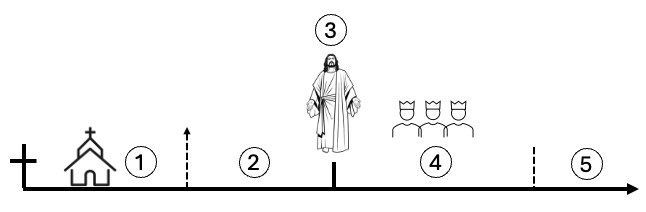
\includegraphics[width=\textwidth]{images/premillennialism.png}
    \caption{Premillennialism}
    \label{fig:premillennialism}
\end{figure}

According to the premillennial view, the sequence is:

\begin{itemize}
\item[\ding{172} ] the Church Age, 
\item[\ding{173} ] a period of great tribulation. 
\item[\ding{174} ] Jesus Christ returns. 
\item[\ding{175} ] the Millennium starts and the saints reign with Christ. 
\item[\ding{176} ] God brings forth the new heaven and the new earth.
\end{itemize}



\section*{Postmillennialism}

According to the postmillennial view, the sequence begins with \ding{172} the Church Age, followed by \ding{173} the Millennium. After this period, \ding{174} Jesus Christ returns, and finally \ding{175} God brings forth the new heaven and the new earth.

\begin{figure}[htbp]
    \centering
    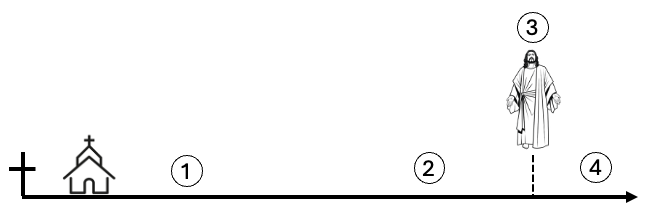
\includegraphics[width=\textwidth]{images/postmillennialism.png}
    \caption{Postmillennialism}
    \label{fig:postmillennialism}
\end{figure}

\section*{Amillennialism}

According to the amillennial view, \ding{172} the present Church Age is itself the Millennium. The thousand years are understood symbolically, representing Christ's present reign rather than a separate, future thousand-year kingdom on earth. At the close of this age, \ding{173} Jesus Christ returns, and \ding{174} God brings forth the new heaven and the new earth.

\begin{figure}[htbp]
    \centering
    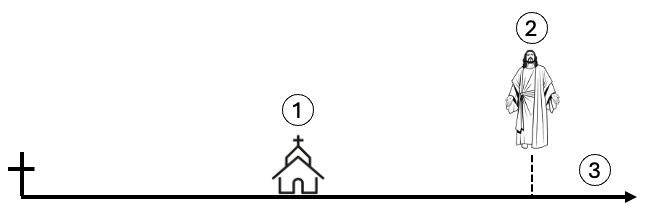
\includegraphics[width=\textwidth]{images/amillennialism.png}
    \caption{Amillennialism}
    \label{fig:amillennialism}
\end{figure}

\begingroup
\small
\renewcommand{\arraystretch}{1.1}
\begin{longtable}{
  >{\RaggedRight\arraybackslash}p{0.15\linewidth}
  >{\RaggedRight\arraybackslash}p{0.24\linewidth}
  >{\RaggedRight\arraybackslash}p{0.24\linewidth}
  >{\RaggedRight\arraybackslash}p{0.24\linewidth}}
\caption{A Comparison of the Three Views of the Millennium}
\label{tab:millennium}\\
\hline
\textbf{Topic} & \textbf{Premil.}\footnote{Representative proponents of premillennialism include Justin Martyr, Irenaeus, Tertullian, John F. Walvoord, and Charles Ryrie.} & \textbf{Postmil.}\footnote{Representative proponents of postmillennialism include Jonathan Edwards, Charles Hodge, and R. C. Sproul.} & \textbf{Amil.}\footnote{Representative proponents of amillennialism include Augustine, John Calvin, and G. K. Beale.} \\
\hline
\endfirsthead

\multicolumn{4}{l}{\footnotesize\itshape Table~\thetable\ (continued)}\\
\hline
\textbf{Topic} & \textbf{Premil.} & \textbf{Postmil.} & \textbf{Amil.} \\
\hline
\endhead

\hline
\multicolumn{4}{r}{\footnotesize\itshape Continued on next page}\\
\endfoot

\hline
\endlastfoot

Christ's return &
Before the Millennium &
After the Millennium &
After the Millennium, understood as the Church Age \\

The Millennium &
A literal thousand-year reign of Christ on earth following His return &
A period in which the gospel advances powerfully throughout the world, bringing widespread conversion, righteousness, and peace; generally understood symbolically rather than as a literal thousand years &
The Church Age, represented by a symbolic thousand years, during which Christ reigns now in heaven \\

Satan's binding &
Released for a short time at the end of the thousand years, then thrown into the lake of fire &
Greatly restrained so that he cannot prevent the gospel from reaching the nations; his binding is understood to occur before or during the Millennium &
Restrained from preventing the gospel from reaching the nations, though he remains active in opposing God's people \\

The resurrection &
Two stages: believers are raised before or at the beginning of the Millennium; unbelievers are raised afterward for judgment &
A general resurrection of both believers and unbelievers at Christ's return &
As in postmillennialism: a general resurrection of both believers and unbelievers at Christ's return \\

The final rebellion &
After the Millennium &
Near the end of the Millennium &
At the close of the present age \\
\end{longtable}
\endgroup